\chapter{Transmissão Elétrica}
\localtableofcontents 

Este capítulo é baseado nas notas de aula do curso, ministrado em 14/08/2023 e 16/08/2023, e no capítulo 14 de \textcite{cretì_fontini_2019}.

Até o momento ignoramos completamente o aspecto de transmissão do nosso modelo de despacho ótimo, no sentido que sempre assumimos implicitamente que a transmissão era eficiente e capaz de atender tanto demanda quando oferta de eletricidade. A partir deste momento, consideramos essas restrições de transmissão no modelo.

\section{Despacho Ótimo com Restrições de Transmissão e Preços Nodais}
Adicionar a rede de transmissão implica perguntar como essa rede deve ser precificada. O modelo desta sessão visa explicar esse ponto. Segue uma importante definição:
\begin{defin}[Preços Nodais]
    São os preços que permitem atingir, de forma descentralizada, a solução do problema de despacho de energia ótimo (na rede) maximizador de bem-estar.
\end{defin}

 Nesse contexto, o despacho ótimo de um sistema é a quantidade líquida que deve ser injetada e retirada em cada nó de forma a maximizar o bem-estar social, para uma determinada carga e características técnicas, econômicas e locacionais da geração e transmissão de energia. Portanto, o despacho ótimo representa a alocação que seria decidida por um OS benevolente, perfeitamente informado e exclusivamente preocupado com a eficiência do sistema, mas livre de qualquer preocupação distributiva.

Nesse modelo existe a suposição implícita que todas as usinas no
mesmo nó são pagas o preço uniforme local, associado a esse nó; o mesmo é verdade para a carga. Vamos exemplificar o modelo com o caso mais simples possível.

Suponha a rede seja composta de dois nós tal que em um deles estejam as usinas e no outro os consumidores (carga). Suponha, mais ainda, que só exista uma usina, indexada por $i$. Teremos então que a solução maximizadora de bem-estar é dada por:
\begin{align*}
    \max_{q^d,q_i}&\quad U(q^d)-c(q_i)\\
    \text{s.a.}&\quad q^d=q_i\\
    &\quad q_i\le k^{max}\\
    &\quad 0\le q_i\le q_i^{max}\\
    &\quad 0\le q^n \le q^{n^{max}}
\end{align*}
Implicando o seguinte Lagrangiano:
\begin{align*}
    \mathcal{L} = c(q_i)-U(q^d)+\mu(q_i-q_d)+\chi(q_i-k^{max}) - \lambda_1q_i + \lambda_2(q_i-q_i^{max}) - \lambda_3q^n + \lambda_4(q^n-q^{n^{max}})
\end{align*}
Implicando as CPOs:
\begin{align*}
    \frac{\partial\mathcal{L}}{\partial q_i} &= c'(q_i) +\mu +\chi -\lambda_1+\lambda_2 = 0 \Rightarrow -\mu = c'(q_i)+\chi-\lambda_1 + \lambda_2 \\ 
    \frac{\partial\mathcal{L}}{\partial q^d} &= - U'(q^d) - \mu -\lambda_3+\lambda_4=0 \Rightarrow -\mu = U'(q^d) + \lambda_3-\lambda_4
\end{align*}
E condições de frouxidão complementar:
\begin{align*}
    \mu(q_i-q_d)=\chi(q_i-k^{max}) =\lambda_1q_i =\lambda_2(q_i-q_i^{max})=0
\end{align*}
Além das factibilidades primais e duais. Note, inclusive, que só há congestionamento na transmissão se $q_i=k^{max}$, implicando $\chi>0$. Portanto, $\chi$ representa o valor da linha de transmissão entre os dois nós. Mais ainda, a linha de transmissão só tem valor econômico se houver congestionamento. Desta proposição inferimos que na ausência de congestionamento, teremos CPOs idênticas ao problema visto no Capítulo~2, levando, portanto, a resultados idênticos.

Repare que o problema discutido acima é referente ao planejador central. Naturalmente, sabemos que em um mercado perfeitamente competitivo valerá o Primeiro Teorema do Bem-Estar, implicando equivalência de alocações sob $p=c'(q_i^*)$, na solução interior. Entretanto, conforme discutido anteriormente, caso exista congestionamento na transmissão teremos 
\[p=c'(q_i^*)+\chi\] 
a definição analítica do preço nodal. Logo, se existem diferentes preços entre diferentes nós, sabemos que há congestionamento no sistema.

\section{Múltiplos Nós}
Pode parecer imediata a extensão do exemplo de dois nós, visto na seção anterior, para o caso de múltiplos nós. Isso não é verdade, entretanto, em virtude das características físicas do processo de transmissão de energia - nomeadamente, das chamadas Leis de Kirkoff.

Aqui, resolverei o caso de uma rede com 3 nós - que pode ser mais facilmente generalizado em diferentes contextos. Suponha uma rede na qual cada nó produz e demanda eletricidade em diferentes quantidades com diferentes tecnologias. 

As redes estudadas nesta seção formam um "loop". Esse tipo de configuração é referido como "malha". Seja $f_{j,k}$ o fluxo de eletricidade entre quaisquer nós $j$ e $k$. Suponha que a malha seja tal qual um triângulo equilátero. 

\subsection{Caso Específico}
A Figura~\ref{fig:3_nodes} denota o exemplo graficamente.
\begin{figure}
    \centering
    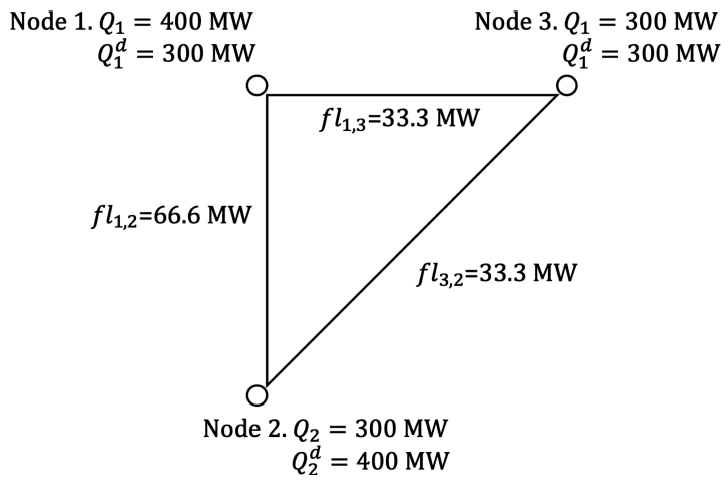
\includegraphics[scale=.4]{figure/mult_nos.png}
    \caption{Exemplo com 3 Nós - Específico}
    \label{fig:3_nodes}
\end{figure}
Teremos que a resistência do trecho $f_{1,3,2}$ é o dobro do trecho $f_{1,2}$ em virtude das distâncias. Mais ainda, sabemos que o nó 1 exporta 100 MW para o nó 2. As Leis de Kirkokff implicam:
\begin{align*}
    \begin{cases}
        f_{1,2}+f_{1,3,2}=100\\
        f_{1,2} = 2f_{1,3,2}
    \end{cases} \Rightarrow (f_{1,2},f_{1,3,2})\approx(66.6,33.3)
\end{align*}
Ora, a existência de equilíbrio depende das restrições de capacidade de transmissão. Suponha que a restrição de capacidade só possa ser ativa em $f_{1,2}$. O problema de maximização de bem-estar (simplificado) pode ser escrito como:
\begin{align*}
    \max_{q_1,q^d}&\quad U(q^d)-c_1(q_1)\\
    \text{s.a.}&\quad q_i=q^d\\
    &\quad 0\leq q_i\leq q_i^{max}\\
    &\quad f_{1,2}\le k^{max} \\
    &\quad f_{1,2}+f_{1,3,2}=100\\
    &\quad f_{1,2} = 2f_{1,3,2}
\end{align*}
Podemos simplificar as últimas 3 restrições para $\frac{2}{3}q_1\le k^{max}$. Escrevendo o Lagrangiano tal qual usual, teremos CPO:
\begin{align*}
    \frac{\partial\mathcal{L}}{\partial q_i} &= c_1 +\mu +\frac{2}{3}\chi -\lambda_1+\lambda_2 = 0 \Rightarrow -\mu = c_1+\frac{2}{3}\chi-\lambda_1 + \lambda_2
\end{align*}
Ou seja, o preço nodal é reduzido. Mais ainda, se $k^{max}=50$, naturalmente, será impossível chegar ao equilíbrio maximizador de bem-estar.

\subsection{Caso Geral}
De forma mais geral, o exemplo acima pode ser definido tal qual indicado na Figura~\ref{fig:3_nodes_gen}. Repare que o problema em questão pode ser escrito como (supondo solução interior):

\begin{figure}
    \centering
    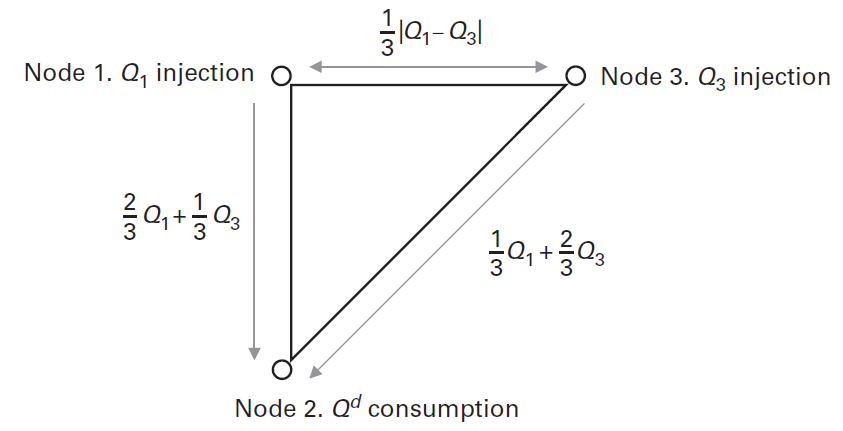
\includegraphics[scale=.4]{figure/3nos.png}
    \caption{Exemplo com 3 Nós - Geral}
    \label{fig:3_nodes_gen}
\end{figure}

\begin{align*}
    \max_{q^d,q_1,q_3}&\quad U(q^d)-c_1q_1-c_3q_3\\
    \text{s.a.}&\quad q^d=q_1+q_3\\
    &\quad\frac{1}{3}|q_1-q_3|\le k^{max}
\end{align*}
Sem perda de generalidade, suponha $q_1\ge q_3$. Teremos um Lagrangiano que implica as seguintes CPOs:
\begin{align*}
    \frac{\partial\mathcal{L}}{\partial q_1} &= 0 \Longrightarrow -\mu = c_1+\frac{1}{3}\chi\\
    \frac{\partial\mathcal{L}}{\partial q_3} &= 0 \Longrightarrow -\mu = c_3-\frac{1}{3}\chi\\ 
    \frac{\partial\mathcal{L}}{\partial q^d} &= 0 \Longrightarrow -\mu =U'(q^d)
\end{align*}
De forma que os preços nodais derivados do equilíbrio descentralizado seriam:
\begin{align*}
    p_1&: p_1\equiv c_1 = p_2 - \frac{\chi}{3}\\
    p_2&: p_2\equiv \lambda = U'(q^d)  \\
    p_3&: p_3\equiv c_3 = p_2 + \frac{\chi}{3}
\end{align*}
Novamente, na ausência de congestionamento os preços serão iguais entre todos os nós e idênticos à utilidade marginal do consumo de eletricidade. Na presença de congestionamento, produção será incentivada no terceiro nó, o mais custoso, mas permite mais geração na usina 1 (mais eficiente) por gerar contrafluxo de eletricidade - aliviando, portanto, o congestionamento da rede. Outra forma de constatar essa externalidade positiva de produção na rede é reparar que, das CPOs:
\begin{align*}
    c_3-c_1=\frac{2}{3}\chi \Longleftrightarrow \chi=\frac{3}{2}(c_3-c_2)
\end{align*}
Isto é, o valor do sistema de distribuição é maior que o diferencial dos custos marginais de produção ou, posto de outra forma, o sistema de distribuição adiciona produtividade na malha. 

Repare, também, que o segundo nó pode estar produzindo eletricidade, entretanto, sua demanda é maior que a oferta e, portanto, precisa importar do resto da rede. O raciocínio para os demais nós vale de forma simétrica. Vamos elaborar sobre essa interpretação na próxima seção.

\section{Expansão de Capacidade}
Suponha um exemplo em que existam dois nós (ou zonas), apenas, com custos marginais diferentes. O exemplo sobre o qual este se baseia está melhor explicitado no Capítulo 14.22 de \textcite{cretì_fontini_2019}. 

Suponha que exista carga e geração em ambas zonas, entretanto, que o custo marginal de produção na zona 1 seja menor que na zona 2. O problema aqui discutido pode ser graficamente representado pela Figura~\ref{fig:zones_1}. 

\begin{figure}
    \centering
    \begin{subfigure}{.45\linewidth}
        \centering
        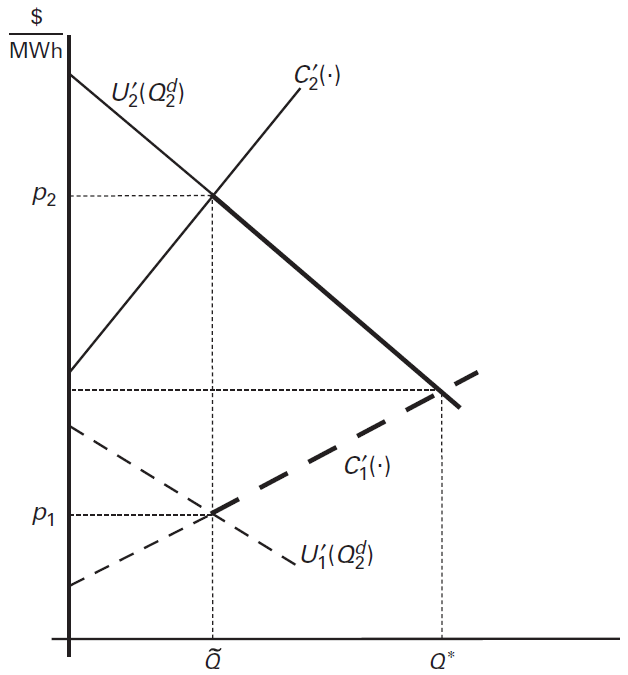
\includegraphics[scale=.3]{figure/zones_1.png}
        \caption{Sem restrições de transmissão}
        \label{fig:zones_1}
    \end{subfigure}
    \begin{subfigure}{.45\linewidth}
        \centering
        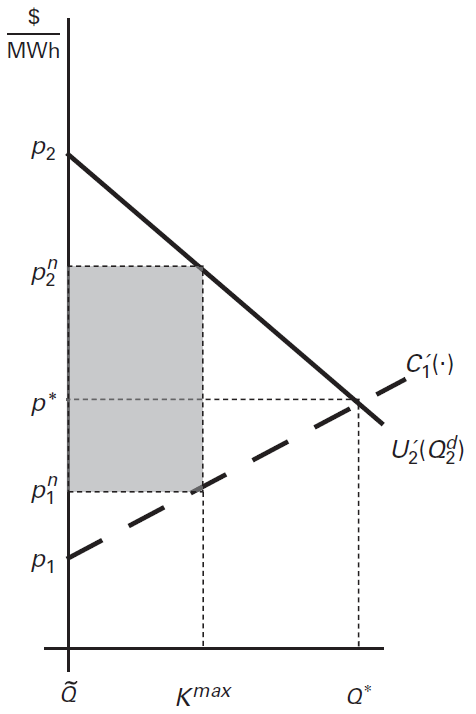
\includegraphics[scale=.3]{figure/zones_2.png}
        \caption{Com restrições de transmissão}
        \label{fig:zones_2}
    \end{subfigure}
    \caption{Problema com Duas Zonas}
\end{figure}

Note que a zona 1, por ser mais eficiente, possibilita a existência de uma demanda adicional na zona 2 que não seria possível caso elas não estivessem conectadas. Desta forma, a zona 1 se torna uma exportadora de energia, enquanto a zona 2 uma importadora.

Suponha, agora, que exista uma restrição de transmissão denotada por $k^{max}$. Note que o problema na zona 2 muda e torna-se tal qual descrito na Figura~\ref{fig:zones_2}. Seja a área sombreada a remuneração do operador pelo uso do sistema de distribuição, de forma similar à seção anterior, denotada por CR (\textit{congestion rent}). 

O bem-estar decorrente \textbf{do fluxo} de energia entre as zonas, considerando a remuneração do operador, pode ser escrito como:
\begin{align*}
    W&= \underbrace{(p_2^n-p_1^n)k^{max}}_{CR}+\underbrace{\frac{1}{2}(p_1^n-p_1)k^{max}}_{PS}+\underbrace{\frac{1}{2}(p_2+p_2^n)k^{max}}_{CS}\\
    &=\frac{(p_2^n-p_1^n)+(p_2-p_1)}{2}k^{max}
\end{align*}
onde PS denota o excedente do produtor (\textit{productor surplus}) e CS o excedente do consumidor (\textit{consumer surplus}).

\subsection{Análise de Bem-Estar}
Note que a existência de congestionamento implica consumo de eletricidade abaixo do ótimo ($k^{max}<q^*$). O próximo passo natural ao economista é mensurar essa perda de bem-estar, chamado de "peso-morto" (\textit{deadweight loss}). Graficamente, ela pode ser compreendida como o triângulo formado entre $k^{max}$ e $q^*$ na Figura~\ref{fig:zones_2}. Analiticamente, definimos:
\[\textit{DWL}(k^{max}) = \frac{1}{2}\Big[\Big(p_2^n(k^{max})-p_1^n(k^{max})\Big)\Big(q^*-q_1(k^{max})\Big)\Big]\]
onde explicitamos as variáveis que são função de $k^{max}$ e $q_1(k^{max})$ é a quantidade exportada da zona 1 para a 2 dado o nível $k^{max}$ de capacidade de transmissão. 

Ora, então o \textbf{operador maximizador de bem-estar} visa minimizar o \textit{DWL}. Esse problema pode ser escrito como:
\begin{align*}
    \min_{k^{max}}\quad \textit{DWL}(k^{max})
\end{align*}
Implicando CPO:
\begin{align*}
    \frac{\partial\textit{DWL}}{\partial k^{max}} = 0 &\Longleftrightarrow \frac{1}{2}\Big[(p_2^{n'}-p_1^{n'})(q^*-q_1)-(p_2^n-p_1^n)q_{1}' \Big]\\
    &\Longleftrightarrow (p_2^n-p_1^n)q_{1}' = (p_2^{n'}-p_1^{n'})(q^*-q_1)
\end{align*}
Sabemos que quando há congestionamento $q_1(k^{max})=q_1=k^{max}$, implicando $q_1'=1$. Portanto, a equação acima simplifica para
\[p_2^n-p_1^n = (p_2^{n'}-p_1^{n'})(q^*-k^{max})\]
Seja $k^{max^*}$ t.q. $k^{max^*}=q^*$, implicando $p_1^n=p_2^n=p^*$. Repare que esse $k^{max^*}$ atende à equação acima. Mais ainda, pelo teorema do valor médio, só existe uma raiz para o polinômio característico da função em questão i.e. só há um valor $k^{max^*}$ que iguala o lado esquerdo ao direito.

Ora, então podemos afirmar que, no ótimo, o operador irá aumentar a capacidade de forma a não haver nenhum peso-morto no sistema, ainda que às custas de sua remuneração - que será 0 no ótimo.

Isso nos indica que, na solução descentralizada, o equilíbrio encontrado será diferente. Analiticamente, observe que o \textbf{problema do operador maximizador de lucro} é dado por:
\begin{align*}
    \max_{k^{max}}\quad \Big(p_2^n(k^{max})-p_1^n(k^{max})\Big)k^{max}
\end{align*}
Implicando CPO:
\[p_2^n-p_1^n=-(p_2^{n'}-p_1^{n'})k^{max}\]
Novamente, pelo teorema do valor intermediário, só existe um $k^{max,SO}$ que resolve a equação acima. Lembre que quando $k^{max}=k^{max^*}$, temos $p_2^n-p_1^n=0\neq -(p_2^{n'}-p_1^{n'})k^{max}$. Portanto, deve ser que $k^{max,SO}<k^{max^*}$.

Isto é, concluímos que no equilíbrio descentralizado haverá menos capacidade que no ótimo - resultado típico de problemas com externalidades positivas.

\subsection{Custos de Expansão}
Suponha, agora, que realizar a expansão seja custoso. Podemos reescrever o \textbf{problema centralizado} como:
\begin{align*}
    \min_{k^{max}}\quad \textit{DWL}(k^{max}) + \underbrace{\beta k^{max}}_{\text{custo da expansão}}
\end{align*}
Implicando CPO:
\[p_2^n-p_1^n = (p_2^{n'}-p_1^{n'})(q^*-k^{max})+2\beta\]
Novamente, só existe um valor $k^{max,\beta}$ que resolve a equação acima. Mais ainda, visto que $\beta>0$, temos que  $k^{max,\beta}<k^{max^*}$ (argumento similar ao da subseção anterior). Portanto, caso existam custos de expansão do sistema de distribuição, haverá \textit{DWL} no ótimo. Repare que podemos reescrever a equação acima como:
\[\frac{1}{2}\Big[p_2^n-p_1^n - (p_2^{n'}-p_1^{n'})(q^*-k^{max})\Big]=\beta\]
Ou seja, o nível ótimo de capacidade será aquele que faz com que o benefício marginal da expansão do sistema de distribuição se iguale ao custo marginal de expandí-lo.

De forma análoga, teremos que o \textbf{problema descentralizado} implica a seguinte CPO:
\[p_2^n-p_1^n+(p_2^{n'}-p_1^{n'})k^{max}=\beta\]
Argumento similar segue, de forma a demonstrar que $k^{max,SO,\beta}$, solução da equação acima, é tal que $k^{max,SO,\beta}<k^{max,SO}<k^{max^*}$. Entretanto, note que nada pode ser dito quando à $k^{max,\beta}$ i.e. $k^{max,SO,\beta}\gtrless k^{max,\beta}$. Ou seja, na presença de custos de expansão, é possível que a solução descentralizada esteja mais próximo do ótimo do que no caso sem custos de expansão. 